\chapter{ML Taxonomy: Map of the Universe}
\label{chap:ml_taxonomy}

% ========================================
% SECTION 0: METADATA
% ========================================
% Prerequisites: None
% Learning Outcomes:
% - Distinguish Supervised, Unsupervised, and RL
% - Understand Regression vs Classification
% - Identify Structured vs Unstructured data
% Interview Relevance: Medium (Foundational context)

% ========================================
% SECTION 1: MOTIVATION
% ========================================
\section{Motivation}
Before diving into algorithms, you need a map. Machine Learning is not a single technique but a collection of tools, each designed for a specific type of problem. Using a hammer (Regression) to tighten a screw (Classification) will only lead to frustration. This chapter defines the landscape so you know exactly which tool to pick.

% ========================================
% SECTION 2: INTUITION
% ========================================
\section{Intuition: The Learning Paradigms}
Imagine you are teaching a child to identify fruits:

\begin{itemize}
    \item \textbf{Supervised Learning} (The Teacher): You hold up an apple and say "This is an apple." You hold up a banana and say "This is a banana." The child learns by mapping images to your labels.
    \item \textbf{Unsupervised Learning} (The Explorer): You give the child a basket of mixed fruits and say nothing. The child groups them by shape and color (clustering)—"these curve yellow/long ones go here, specific round red ones go there." They don't know the names, but they know the patterns.
    \item \textbf{Reinforcement Learning} (The Dog Trainer): You don't give answers or data. The child rides a bicycle. If they fall, it hurts (negative reward). If they balance, they have fun (positive reward). They learn by trial and error.
\end{itemize}

% ========================================
% SECTION 3: VISUALIZATION
% ========================================
\section{Visualizing the Taxonomy}

\begin{figure}[h]
    \centering
    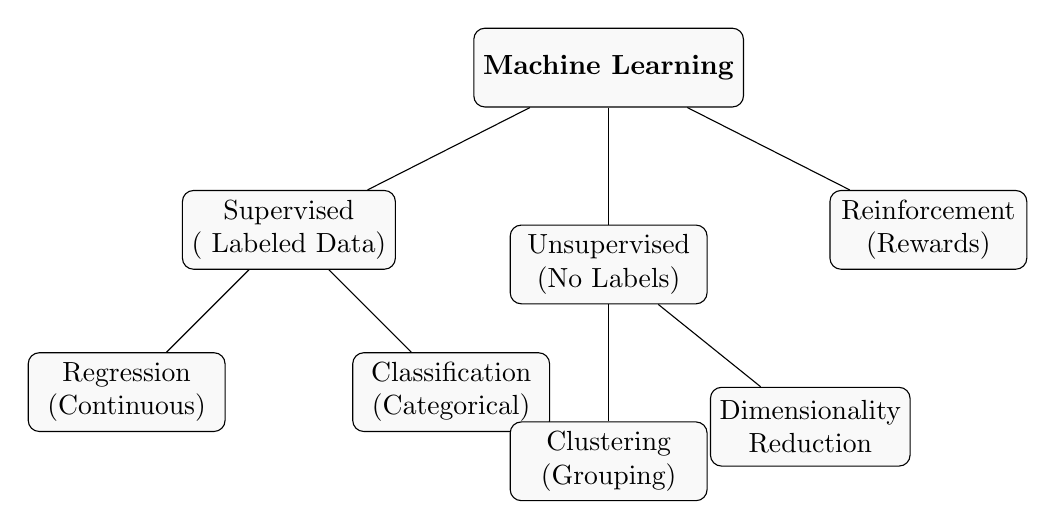
\begin{tikzpicture}[
        node distance=1.5cm,
        every node/.style={rectangle, rounded corners, draw=black, align=center, fill=gray!5, minimum width=2.5cm, minimum height=1cm},
        edge from parent/.style={draw, ->, thick}
    ]
        \node (ml) {\textbf{Machine Learning}};
        
        \node (sup) [below left of=ml, xshift=-3cm, yshift=-1cm] {Supervised\\( Labeled Data)};
        \node (unsup) [below of=ml, yshift=-1cm] {Unsupervised\\(No Labels)};
        \node (rl) [below right of=ml, xshift=3cm, yshift=-1cm] {Reinforcement\\(Rewards)};
        
        \node (reg) [below left of=sup, xshift=-1cm, yshift=-1cm] {Regression\\(Continuous)};
        \node (cls) [below right of=sup, xshift=1cm, yshift=-1cm] {Classification\\(Categorical)};
        
        \node (clust) [below of=unsup, yshift=-1cm] {Clustering\\(Grouping)};
        \node (dim) [below right of=unsup, xshift=1.5cm, yshift=-1cm] {Dimensionality\\Reduction};
        
        \draw (ml) -- (sup);
        \draw (ml) -- (unsup);
        \draw (ml) -- (rl);
        \draw (sup) -- (reg);
        \draw (sup) -- (cls);
        \draw (unsup) -- (clust);
        \draw (unsup) -- (dim);
    \end{tikzpicture}
    \caption{The Machine Learning Landscape. This book focuses strictly on the left branch: \textbf{Supervised Learning}.}
    \label{fig:ml_taxonomy}
\end{figure}

% ========================================
% SECTION 4: DEFINITIONS
% ========================================
\section{Key Definitions}

\subsection{1. Supervised Learning}
\textbf{Goal}: Learn a mapping function $f: X \rightarrow y$.
\begin{itemize}
    \item \textbf{Input ($X$)}: Features, Independent variables (e.g., Age, Income).
    \item \textbf{Output ($y$)}: Target, Label, Dependent variable (e.g., Loan Approved?).
    \item \textbf{Data}: We need pairs of $(X, y)$.
\end{itemize}

\subsection{2. Regression vs Classification}
Within Supervised Learning, the distinction depends on the \textbf{Data Type of the Target ($y$)}:
\begin{itemize}
    \item \textbf{Regression}: $y$ is \textbf{Continuous} (Numbers).
    \begin{itemize}
        \item Examples: Price ($100k, 105k$), Temperature ($25^\circ C$), Height.
        \item Algorithms: Linear Regression, Random Forest Regressor.
    \end{itemize}
    \item \textbf{Classification}: $y$ is \textbf{Categorical} (Classes/Labels).
    \begin{itemize}
        \item Examples: Spam/Not Spam (Binary), Cat/Dog/Mouse (Multiclass).
        \item Algorithms: Logistic Regression, SVM, Decision Trees.
    \end{itemize}
\end{itemize}

% ========================================
% SECTION 5: STRUCTURED VS UNSTRUCTURED
% ========================================
\section{Data Types}
\begin{enumerate}
    \item \textbf{Structured (Tabular)}: Excel sheets, SQL tables. Rows and columns.
    \item \textbf{Unstructured}: Images, Audio, Text, Video. No predefined table structure.
    \item \textbf{Time-Series}: Data indexed by time (Stock prices, weather).
\end{enumerate}

% ========================================
% SECTION 6: IMPLEMENTATION
% ========================================
\section{Python: Identify Your Problem}
\begin{lstlisting}[language=Python, caption=Distinguishing Targets]
import pandas as pd

df = pd.read_csv("data.csv")
target = df['y']

# Check number of unique values
num_unique = target.nunique()

if target.dtype == 'object' or num_unique < 20:
    print("Likely CLASSIFICATION")
    print(f"Classes: {target.unique()}")
else:
    print("Likely REGRESSION")
    print(f"Range: {target.min()} to {target.max()}")
\end{lstlisting}

% ========================================
% SECTION 7: PRACTICAL CONSIDERATIONS
% ========================================
\section{Pitfalls}
\begin{itemize}
    \item \textbf{Framing Errors}: Trying to predict "Rating (1-5)" as Regression? It's often better as Ordinal Classification.
    \item \textbf{Data Leakage}: Using future data (features created after the event) to predict the event.
    \item \textbf{Semi-Supervised}: When you have 1000 images but only 100 labels. Don't discard the 900 unlabeled ones!
\end{itemize}

% ========================================
% SECTION 8: INTERVIEW QUESTIONS
% ========================================
\section{HOTS Questions}
\textbf{Q1: Is Logistic Regression a Regression algorithm?}
\begin{itemize}
    \item No. Despite the name, it is a \textbf{Classification} algorithm. It predicts probabilities (continuous 0-1) but uses a threshold to output a class.
\end{itemize}

\textbf{Q2: What is the difference between Supervised and Unsupervised Learning?}
\begin{itemize}
    \item Supervised: Known labels ($y$). Goal is prediction.
    \item Unsupervised: No labels. Goal is structure/pattern discovery.
\end{itemize}

% ========================================
% SECTION 9: QUICK REFERENCE
% ========================================
\section{Quick Reference Card}

\begin{center}
\fbox{\parbox{0.9\textwidth}{
\textbf{ML TAXONOMY - CHEAT SHEET}
\vspace{0.3cm}

\textbf{3 Primary Paradigms}:
\begin{enumerate}
    \item \textbf{Supervised}: $X \rightarrow y$ (Prediction). Has Labels.
    \item \textbf{Unsupervised}: $X \rightarrow ?$ (Pattern Finding). No Labels.
    \item \textbf{Reinforcement}: Agent $\rightarrow$ Action $\rightarrow$ Reward.
\end{enumerate}

\textbf{Supervised Breakdown}:
\begin{center}
\begin{tabular}{|l|l|l|}
\hline
\textbf{Type} & \textbf{Target ($y$)} & \textbf{Examples} \\ \hline
Regression & Continuous Number & House Price, Temp \\ \hline
Classification & Categorical Label & Spam, Fraud, Disease \\ \hline
\end{tabular}
\end{center}

\textbf{Interview Gold}:
\begin{itemize}
    \item "Regression" vs "Classification" depends on the TARGET, not the input.
    \item Discrete numbers (e.g., number of children) can be treated as Regression (Count regression) or Classification depending on range.
\end{itemize}
}}
\end{center}
